前一章讨论了如何将波场向下外推,进行外推处理很简单,因为它只不过是在频率域内
用$\exp[ik_z(\omega,k_x)z]$来乘而已。有限差分法则较复杂,这将涉及新的近似和新的陷阱。
我们为何要自寻烦恼去学习它呢?首先,许多人发现有限差分方法更易于理解,在时间空间
域$(t,x,z)$内,没有复数,没有复指数,也没有称为FFT
(快速傅氏变换)的“魔盒”。

情况类似于在普通的频率滤波中所遇到的情形。频率滤波可以作为频率域内的某种乘积
或者时间域内的某种褶积来完成,而波场外推则既有与时间有关的频率域$\omega$内的乘积又有与空
间有关的波数域$k_x$内的乘积。新因素就是二维$(\omega,k_x)$空间,它代替了旧有的一维$\omega$空间。
关于为什么要自找麻烦去利用有限差分这个问题,其实是一个涉及为何要采用二维形式的老
问题:在已经发现快速傅氏变换以后,为什么还要用时间域滤波运算去自找麻烦呢?

在许多场合下还会多次提出这个问题。以后我们还会有炮检距坐标轴和共中心点坐标
轴,所以我们还需要选择究竟是在这些坐标上应用有限差分法呢还是采用傅氏变换。这不是
一种要么全是要么全非这样的命题:不是必须选择傅氏变换,就是必须选择褶积(有限差
分)。

这个问题的答案是多方面的,正如地球物理目标是多方面的一样。判断该问题答案是否正
确的准则大多数是从普通的滤波理论中所早已熟知的。那些电气工程师和曾经强迫自己涉足
波动处理领域的老式反褶积专家到头来是要为这一点而深感高兴的,他们未曾料到他们的知
识竟已经有了这么多方面的应用。

图\ref{fig:txz/freqhyp}说明傅氏变换域计算与时间域计算之间的差异。为突出显示各个域内都有难点,
该图是在一种$256\times64$的网格上计算出来的。一般来说,你可注意到在傅氏域计算中有假频干
扰,在时间域计算中有频散(见\label{sec:4.3}节)。(图\ref{fig:txz/freqhyp}中的所谓“时间域”双曲线实际上就
是频率域情形的一种重复模拟——将整个双曲线叠合起来进入视界)。在本章中,我们将会知
道如何去完成时间域计算,各个域内计算结果的更详细比较在第四章内进行。
\begin{figure}[H]
\centering
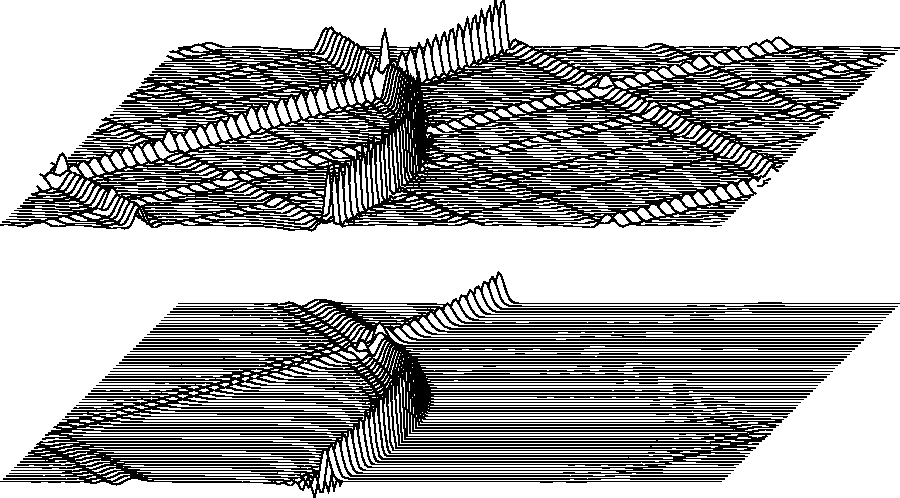
\includegraphics[width=0.95\textwidth]{txz/freqhyp}
\caption[freqhyp]{频率域双曲线(上图)与时间域双曲线(下图)}
\label{fig:txz/freqhyp}
\end{figure}

即使你经常在频率域内作偏移处理,为有助于你选择参数以获得良好时间域响应,研究
一下时间域方法还是值得的。例如,图\ref{fig:txz/freqhyp}的上、下两部分都是在频率域内完成的,但是
为获得更合理的响应,有一种是模拟时间域计算的。
\subsection{横向变化}
在通常的线性滤波理论中,一个滤波器可以成为时变的,这点在反射地震学中很有
用,因为回声反射的频率成分就是随时间而改变的。时变滤波的一个恼人问题是不能用频率
域内的简单乘积关系描述它,所以在时变滤波是单独应用时,就得放弃频率域,或者,就得构
造出所有类型的畸变(例如,对时间坐标轴进行拉伸)以便显得像是时变的。

所有这些考虑同样也适用于水平空间坐标二关于空间坐标,还涉及一个新问题,这就
是地震波速度$v$。如果速度是空间可变的,例如是$v(x)$,则向上和向下外推波场的运算就
不能表示为$k_x$域内的乘积关系了,进行波场外推必须放弃空间频率域而采用有限差分。为显
得像是空间可变(space-invariant),可供选择的办法再一次又是构造一切类型的畸变(诸
如对$x$轴进行拉伸之类)。

在二维或二维以上的情形下,进行拉伸处理会变得更困难而且很少能令人满意。

建议采用有限差分而不采用傅里叶变换方法。还有一种问题类型相同但情况不那么严峻
的原因,那就是记录道位置的空间横向变动。如检波器由于某种原因变成了不规则分布,致
使记录道间距$\Delta x$不是与$x$无关,这时就只有两种办法可供选择了 :
\begin{enumerate}
\item 在进行傅里叶分析
之前,以均匀间隔对数据进行重采样;
\item 用有限差分直接处理资料。
\end{enumerate}

\subsection{时差}
许多地震学方法是进行时移测定。时差(Stepout)
一词表示旅行时间随位置之改变而
发生的变化。通常频率域的计算结果最后都要变换至时伺域,以便时移清楚可见。时间域计
算的好处就是:在进行计算时就可以测定波束的时移。在频率域内,确定一个时间参考点或者
描述整个时间函数的时间偏移倒并不困难,但是不变换返回时间域就想存取单独的子波或波
束就没那么容易。

上行波场和下行波场的外推滤波因子、即$\exp[ik_z(\omega,k_x)z]$,基本上是一种物理可
实现全通滤波(在某些情形下,它是非物理可实现的),它可以完成能量偏移而无放大或阻
尼作用,我想这就是为什么偏移滤波比极小相位滤波更有意思的原因。偏移滤波遍及所有空
间采集能量而后置于恰当的位置上,而极小相位滤波则完全难以使能量偏移,它们只不过
是使某些频率成分放大而使另外一些频率成分缩小而已。任何形式为$\exp[i\phi(\omega)]$的滤波因
子都是一种全通滤波(all-pass filter),那么,欲使$\exp (i\phi)$的时间域表现形式具有物
理可实现性,函数$\phi(\omega)$到底应有什么约束条件呢?

物理可实现全通滤波具有一种颇引人注意的表现形式,用Z变换来描述,就是具有
$Z^N\overset{-}{A}(l/Z)/A(Z)$形式。熟悉滤波理论的人都会理解,用来除要涉及到一系列新
问题:反馈、参量简化以及可能的不稳定性(见\ref{sec:4.6}节关于Z变换的讨论)。在采用有限差
分进行波场向下外推时,同样也会引起所有这些问题。向下外推就是一个反馈过程。参量简
化是颇引人入胜的,设取$A(Z)=1+a_1Z+a_2Z^2$,有两个可调节的系数就足以为有选择的延
迟选出适当的频率和频带宽度了。参量简化也意味着应用时很省事,这点是很妙的。很妙的
还有:所具有的函数形式本身就意昧着具有物理可实现性。另一方面,节省时间所能带来的
好处会被若干危险因素所抵销,所以我们现在必须熟悉并利用某种稳定性定理,必须假定
是极小相位的。

\subsection{频率域内消除干扰要求过苛}
傅里叶方法是整体性方法,就是说,在可以开始进行处理之前,必须掌握有全部数据
组。间接误差与截断误差可能具有严重的局部影响。另一方面,有限差分方法则是局部性方
法,各数据点仅与其邻点直接有关,间接误差传播缓慢。让我们在一维时间序列分析方面举
出两个有关频率域隐藏危险的例子。

在频率域内很容易设计锐截止滤波因子,例如,设计成在8赫兹至80赫兹之间有一绝对平
坦的通频带而在其外则一律为零。但这类滤波因子在时间域内却引起了问题,它们必然是非
物理可实现的,即在能量输入于滤波器之前就产生响应。另一个糟糕的问题是时间响应只随
时间t反比衰减。这样一来,振幅已按时间平方反比衰减的到达较迟之深反射就将被较早到
达之反射所引起的长长的滤波响应所淹没。

更常见的问题是由抑制60周动力线频率的滤波器引起的,许多记录设备中均有这类滤波
器。在Z变换域内很容易设计这类陷频滤波器,只需在单位圆上准确等于60周之处有一个零
点即可。这种滤波器可消除60周干扰,但是它却会在其他频率上使通频带畸变。因此,需要
在单位圆之外稍远的地方置一极点。极点与零点之间的间距决定了陷频的频带宽度。如从单
位圆周上某种距离之处来观察这一对点时,该极点就具有几乎将零点影响完全消除的作用。
因此,远离抑制带就有理想的平缓频谱。你就用这种滤波器来记录某种数据。由于到达晚的
反射均比到达早的一些反射要弱些,所以,显示绘图程序就得随时间而增大其增益。但在接
入你的陷频滤波器后,你会发现这种滤波器使动力线干扰增大了而不是减弱了。为什么?原
因就在于你企图过于干净地消除干扰而使极点过于靠近零点了。指数增益实际上使单位圆远
离零点而移向极点,于是极点也许就落在了单位圆上!使极点远离零点可形成一种比较开阔
的陷频带,在频率域内设计滤波器时,这点是不受欢迎的,但是当增益随时间而变动时,这
种滤波器至少会工作得比较灵敏。

\subsection{填补零值点}
开始应用快速傅氏变换时,首先是应用于褶积。如果一个滤波因子有多于五十项左右的
系数,用频率域内的乘法来实现该项滤波处理,运算速度会比较快一些。如已经谨慎地用足
够的零值点填满了数据与滤波因子的尾端部分,这种运算结果将与褶积结果完全相同。填补
零值点使离散傅氏变换的周期性质被掩盖起来而不露痕迹。对典型长度约为一千个采样点的
时间函数进行滤波时,为了节省计算时间,宁可稍许增加一些内存,而地震剖面都是有上千
记录道之长的。对于偏移运算,必须同时在空间轴与时间轴上完成零值点的填补。可能需要
补零的有三处,如下所示:
\begin{table}[!ht]
\centering
\ttfamily
\small
\begin{tabularx}{\textwidth}{|Y|Y|}
%\begin{tabular}{p{3cm}p{4cm}p{4cm}p{5cm}}
%\toprule
\hline
 数据& 0 \\
%\midrule
\hline
0&0\\
\hline


%\bottomrule
\end{tabularx}
%\end{tabular}
\end{table}
在\ref{sec:4.5}节内将对如何减轻频率域偏移的麻烦问题有所提示。

\subsection{展望}
频率域内的一些问题已在上面总结过了,在这一章和第四章内,将要指出空间域内存在
的一些问题。地震数据处理是一种多维的处理任务,而不同的维数往往要用不同的方法去处
理。不过,如果你确信你对于频率域处理有把握,那么,你可以将这章的很多部分跳过而直接
去阅读第三章。在该章中,你可学习到有关炮检距、叠加及叠前偏移等问题。
